\documentclass{article}

\usepackage{graphicx}
\usepackage{tikz}
\usepackage{tikzsymbols}
\usetikzlibrary{calc,patterns,shapes.geometric}
\pagestyle{empty}
\usepackage[margin=0pt]{geometry}
\geometry{papersize={14in,12in}}

\def\centerarc[#1](#2)(#3:#4:#5){\draw[#1] ($(#2)+({#5*cos(#3)},{#5*sin(#3)})$) arc (#3:#4:#5);}

\begin{document}
	\begin{figure}
		\centering
		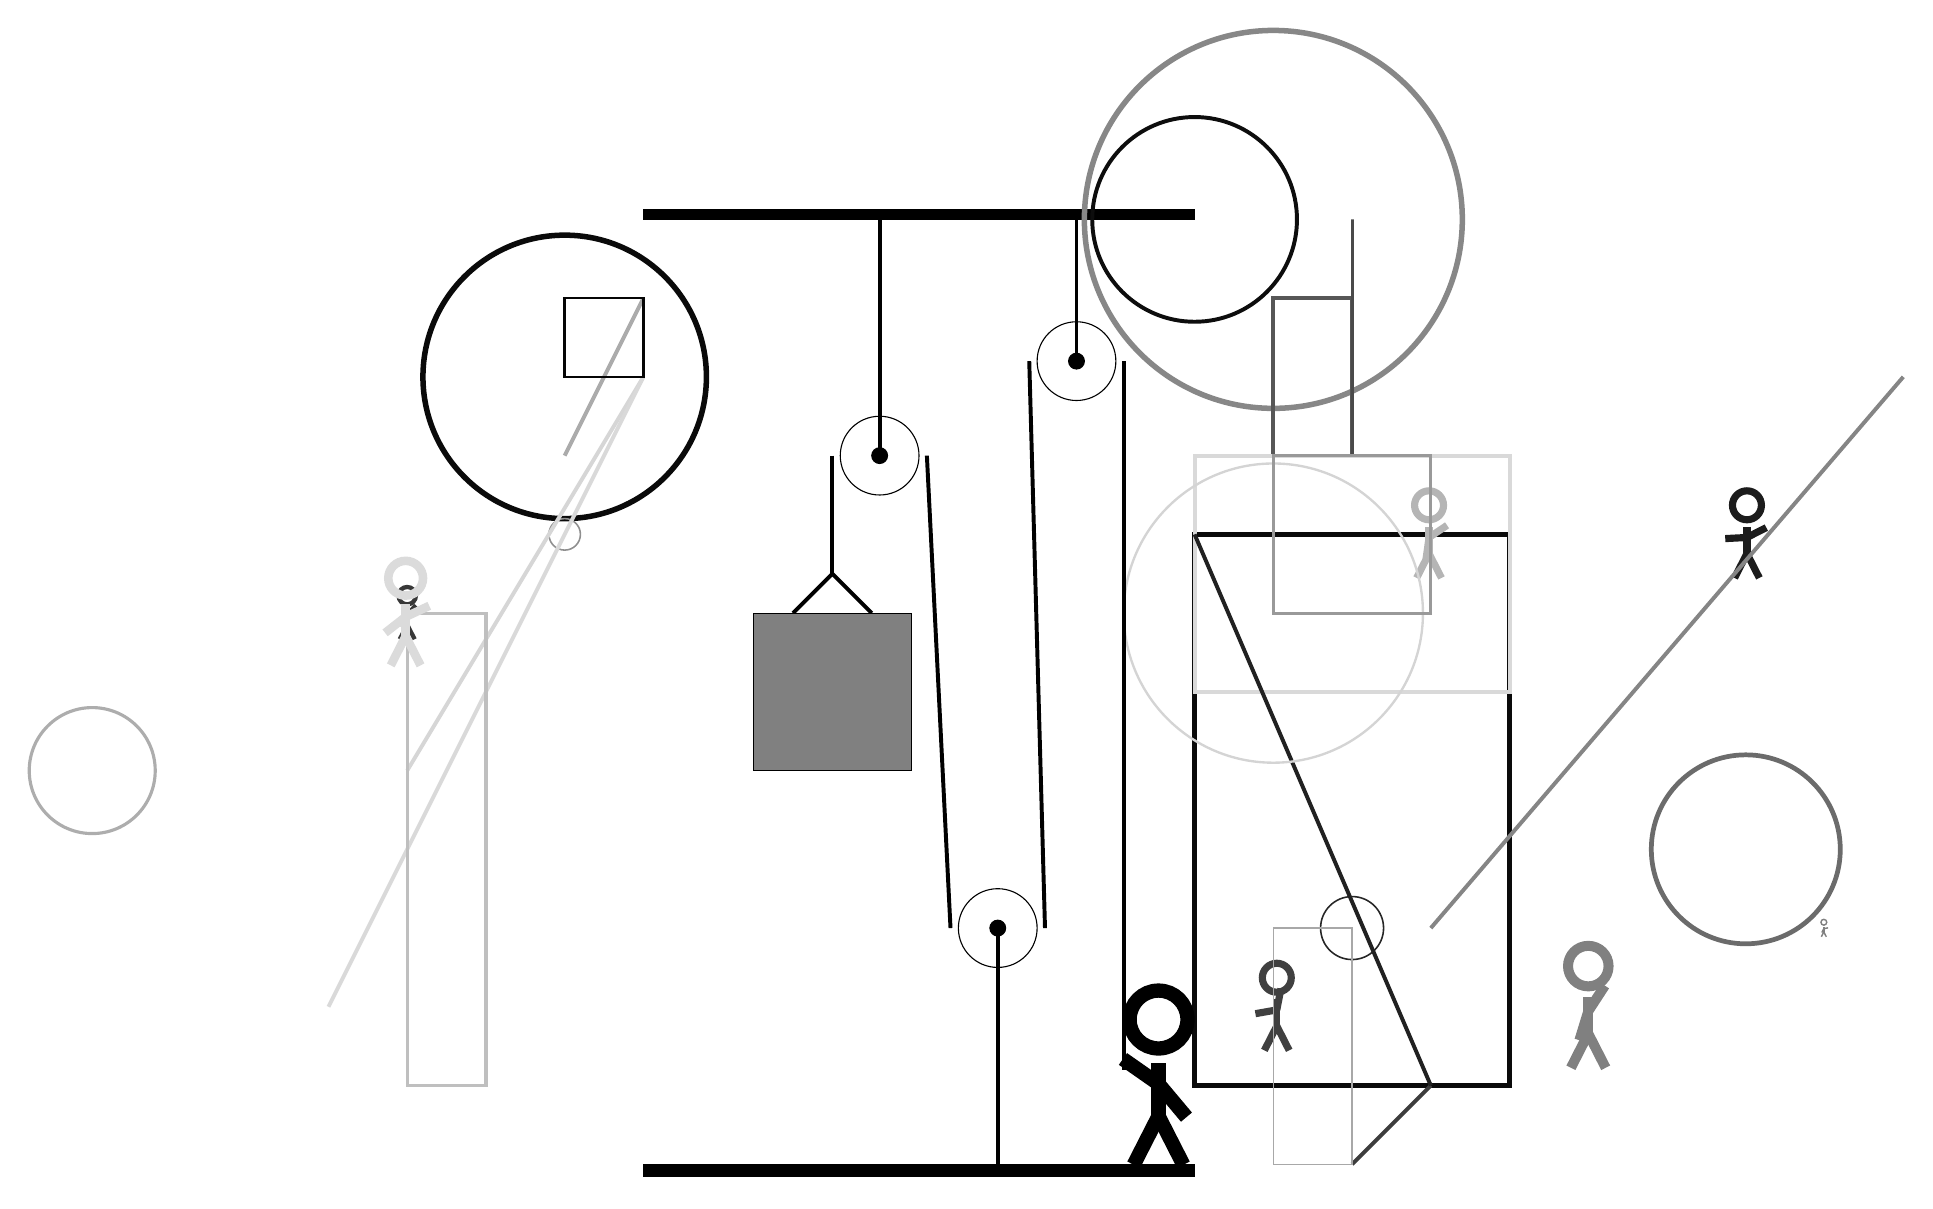
\begin{tikzpicture}
			%%%%% START %%%%%
			
			\draw[fill=black] (-2, 9) rectangle (5, 9.125);
			
			\draw (1, 6) circle (0.5);
			\draw[fill=black] (1, 6) circle (0.1);
			\draw[line width=0.5mm]  (1, 9) -- (1, 6);
			
			\draw[fill=white](2.5, 0) circle (0.5);
			\draw[fill=black] (2.5, 0) circle (0.1);
			\draw[line width=0.5mm]  (2.5, -3) -- (2.5, 0);
			
			\draw [line width=0.7mm, color=black!47](6, 9) circle (2.4);
			
			\draw [line width=0.7mm, color=black!96](-3, 7) circle (1.8);
			\draw[line width=0.5mm, color=black!66] (6, 6) rectangle (7, 8);
			\draw[line width=0.7mm, color=black!96] (5, -2) rectangle (9, 5);
			\draw[line width=0.5mm, color=black!33](-2, 8) -- (-3, 6);
			\node[line width=0.7mm, color=black!29] at (8, 5) {\Strichmaxerl[5][82][34]};
			\draw [line width=0.2mm, color=black!85](7, 0) circle (0.4);
			
			\node[line width=0.4mm, color=black!50] at (10, -1) {\Strichmaxerl[7][73][57]};
			\node[line width=0.3mm, color=black!78] at (-5, 4) {\Strichmaxerl[3][50][49]};
			
			\draw [line width=0.2mm, color=black!44](-3, 5) circle (0.2);
			\node[line width=0.5mm, color=black!75] at (6, -1) {\Strichmaxerl[5][10][79]};
			
			\draw[line width=0.5mm, color=black!16](-5, 2) -- (-2, 7);
			\draw[line width=0.5mm, color=black!76](7, -3) -- (8, -2);
			
			\draw[line width=0.5mm, color=black!15](-6, -1) -- (-2, 7);
			\draw[line width=0.5mm, color=black!15] (5, 6) rectangle (9, 3);
			\node[line width=0.7mm, color=black!89] at (12, 5) {\Strichmaxerl[5][3][27]};
			
			\draw[line width=0.5mm, color=black!48](8, 0) -- (14, 7);
			
			\draw[line width=0.4mm, color=black!71] (7, 9) rectangle (7, 6);
			\draw[line width=0.4mm, color=black!25] (-4, 4) rectangle (-5, -2);
			
			\draw[line width=0.5mm, color=black!87](5, 5) -- (8, -2);
			\draw [line width=0.4mm, color=black!32](-9, 2) circle (0.8);
			
			\draw [line width=0.6mm, color=black!58](12, 1) circle (1.2);
			\node[line width=0.2mm, color=black!14] at (-5, 4) {\Strichmaxerl[6][38][25]};
			\draw [line width=0.5mm, color=black!95](5, 9) circle (1.3);
			\draw [line width=0.3mm, color=black!17](6, 4) circle (1.9);
			
			\node[line width=0.2mm, color=black!50] at (13, 0) {\Strichmaxerl[1][62][11]};
			\draw[line width=0.2mm, color=black!34] (6, -3) rectangle (7, 0);
			\draw[line width=0.3mm, color=black!98] (-3, 8) rectangle (-2, 7);
			\draw[line width=0.4mm, color=black!40] (6, 4) rectangle (8, 6);
			
			\draw[fill=white](3.5, 7.2) circle (0.5);
			\draw[fill=black] (3.5, 7.2) circle (0.1);
			\draw[line width=0.5mm] (3.5, 9) -- (3.5, 7.2);
			
			\draw[line width=0.5mm] (-0.1, 4.0) -- (0.4, 4.5) -- (0.9, 4.0);
			\draw[fill=black!50] (-0.6, 4.0) rectangle (1.4, 2.0);
			
			\draw[line width=0.5mm] (0.4, 6) -- (0.4, 4.5);
			\centerarc[line width=0.5mm](1, 6)(0:180:0.6);
			\draw[line width=0.5mm](1.6, 6) -- (1.9, 0);
			\centerarc[line width=0.5mm](2.5, 0)(180:360:0.6);
			\draw[line width=0.5mm](3.1, 0) -- (2.9, 7.2);
			\centerarc[line width=0.5mm](3.5, 7.2)(0:180:0.6);
			\draw[line width=0.5mm](4.1, 7.2) -- (4.1, -1.8);
			
			\node at (4.5, -1.9) {\Strichmaxerl[10][-35][-50]};
			
			\draw[fill=black] (-2, -3) rectangle (5, -3.15);
			
			%%%%% END %%%%%
		\end{tikzpicture}
	\end{figure}	
\end{document}